%%%% यह रूपद निशान्त मिश्रा(https://github.com/nishantaMishra) द्वारा रचा गया था। 
% इसे LuaLaTeX द्वारा सङ्कलित किया जाना चाहिए।



\documentclass[10pt,a4paper,twoside]{article}
\usepackage[utf8]{inputenc} % यह अतीव आवश्यक है। मुद्रण करने के लिए यही प्रतीकों का परिज्ञान करता है। यह अक्षरों और प्रतीकों का एक मानक है। Unicode (or Universal Coded Character Set) Transformation Format – 8-bit. इसके अतिरिक्त भी अनेक सम्पुट प्रविष्ट किये जा सकते हैं परन्तु यदि विशेषज्ञान न हो तो इसका प्रयोग सरलता से किया जा सकता है।
\usepackage[top=3.5cm,bottom=3.5cm,left=1cm,right=1cm,columnsep=20pt]{geometry}
\usepackage{multicol}
\usepackage{fontspec}
\usepackage{polyglossia}
\usepackage[hyphens]{url}
\usepackage{titling}
\usepackage{fancyhdr}
\usepackage{amsmath}
\usepackage{afterpage}
\usepackage[dvipsnames]{xcolor}
\usepackage[T1]{fontenc}
\usepackage[hidelinks]{hyperref}
\usepackage{pstricks}
\usepackage{psvectorian}
\usepackage{enumitem}
\usepackage{mathrsfs}

\usepackage[mathscr]{euscript}%इस सम्पुट को प्रविष्ट करने से रोमक अक्षरों के भिन्न प्ररूप लिखना सम्भव हो पाता है यथा, फूरिये रूपान्तरण का F. eu अर्थात् आयलर।
\usepackage{graphicx} % चित्र निविष्ट करने के लिए
\usepackage{geometry} % इससे पृष्ठ-आकार, पृष्ठ-सीमाएँत तथा शीर्ष
\linespread{1.25} % शब्दों के मध्य १.२५ सहस्रिमान की रिक्ति
\setlength{\parindent}{0pt} % यहाँ हमने परिच्छेद के प्रथम अक्षर की पृष्ठ-सीमा से दूरी को निर्धारित किया है। हमने शून्य बिन्दु लिखकर दूरी न रखने का निर्णय लिया है। इसीलिए सकल परिच्छेद परम वाम से आरम्भ होते हैं। (No paragraph indents)
\setlength{\parskip}{1em} % क्रमागत परिच्छेदों के मध्य की दूरी (एक पँक्ति)
\renewcommand{\headrulewidth}{0pt} % शीर्षलेख को रेखा से पृथक् नहीं करना है इसलिए उस रेखा का वरीमन् शून्य बिन्दु परिभाषित कर दिया है।
\geometry{legalpaper, portrait, margin=1in}
\setlength{\headheight}{14.49998pt}



%मुख्य भाषा हिन्दी को परिभाषित किया तथा शोभिका लिपि(https://github.com/Sandhi-IITBombay/Shobhika) का प्रयोग किया गया।
\setmainlanguage[numerals=Devanagari]{hindi}
\newfontfamily\devanagarifont[Script=Devanagari]{Shobhika}
\setmainfont{Shobhika}
\newfontfamily\englishfont[]{Times New Roman}

\fancyhead[L]{{\rightmark}}
\fancyhead[R]{{\leftmark}}
\renewcommand{\headrulewidth}{1.4pt}
\fancyfoot[C]{\textbf{\devanagarifont\devanagaripagenumber{\thepage}}}
\renewcommand{\footrulewidth}{1.4pt}
\pagestyle{fancy}

%%%%%%%%%%%%%%%%%%%%%%%%%%%%%%%%%%
%% पृष्ठ सङ्ख्या, चित्र सङ्ख्या, खण्ड सङ्ख्या तथा समीकरण सङ्ख्या तको देवनागरी अङ्कों में प्रकट करने के लिए 

\makeatletter
\newcommand{\devanagarinumeral}[1]{\expandafter\@devanagarinumeral\csname c@#1\endcsname}
\newcommand{\@devanagarinumeral}[1]{%
  \ifcase#1\or
  १\or २\or ३\or ४\or ५\or ६\or ७\or ८\or ९\or १०\or
  ११\or १२\or १३\or १४\or १५\or १६\or १७\or १८\or १९\or २०\or
  २१\or २२\or २३\or २४\or २५\or २६\or २७\or २८\or २९\or ३०\or
  ३१\or ३२\or ३३\or ३४\or ३५\or ३६\or ३७\or ३८\or ३९\or ४०\or
  ४१\or ४२\or ४३\or ४४\or ४५\or ४६\or ४७\or ४८\or ४९\or ५०\or
  ५१\or ५२\or ५३\or ५४\or ५५\or ५६\or ५७\or ५८\or ५९\or ६०\or
  ६१\or ६२\or ६३\or ६४\or ६५\or ६६\or ६७\or ६८\or ६९\or ७०\or
  ७१\or ७२\or ७३\or ७४\or ७५\or ७६\or ७७\or ७८\or ७९\or ८०\or
  ८१\or ८२\or ८३\or ८४\or ८५\or ८६\or ८७\or ८८\or ८९\or ९०\or
  ९१\or ९२\or ९३\or ९४\or ९५\or ९६\or ९७\or ९८\or ९९\or १००\else
  \@ctrerr\fi
}


\newcommand{\devanagaridecimal}[1]{\expandafter\@devanagaridecimal#1\@nil}
\def\@devanagaridecimal#1.#2\@nil{%
  \devanagarinumeral{#1}.\devanagarinumeral{#2}%
}
\renewcommand{\thesection}{\devanagarinumeral{section}}
\renewcommand{\thesubsection}{\devanagarinumeral{section}.\devanagarinumeral{subsection}}
\renewcommand{\thesubsubsection}{\devanagarinumeral{section}.\devanagarinumeral{subsection}.\devanagarinumeral{subsubsection}}
\makeatother


%%%%%%%%%%%%%%%%%%%%%%%%%%%%%%%%%%%%%%%
% देवनागरी पृष्ठ सङ्ख्या के लिए 
\newcommand{\devanagaripagenumber}[1]{%
  \ifcase\value{page}\or
  १\or २\or ३\or ४\or ५\or ६\or ७\or ८\or ९\or १०\or 
  ११\or १२\or १३\or १४\or १५\or १६\or १७\or १८\or १९\or २०\or
  २१\or २२\or २३\or २४\or २५\or २६\or २७\or २८\or २९\or ३०\or
  ३१\or ३२\or ३३\or ३४\or ३५\or ३६\or ३७\or ३८\or ३९\or ४०\or
  ४१\or ४२\or ४३\or ४४\or ४५\or ४६\or ४७\or ४८\or ४९\or ५०\or
  ५१\or ५२\or ५३\or ५४\or ५५\or ५६\or ५७\or ५८\or ५९\or ६०\or
  ६१\or ६२\or ६३\or ६४\or ६५\or ६६\or ६७\or ६८\or ६९\or ७०\or
  ७१\or ७२\or ७३\or ७४\or ७५\or ७६\or ७७\or ७८\or ७९\or ८०\or
  ८१\or ८२\or ८३\or ८४\or ८५\or ८६\or ८७\or ८८\or ८९\or ९०\or
  ९१\or ९२\or ९३\or ९४\or ९५\or ९६\or ९७\or ९८\or ९९\or १००\else
  \Numberstring{page} 
  \fi
}

%% सूची के अङ्के देवगानरी में प्रकट करने के लिए। यदि प्रलेख में पचास से अधिक चित्र अथवा समीकरण हों तो निम्नवत् सूची का अतिक्रमण करके उसे वाञ्छित सङ्ख्या तक बढ़ा देना चाहिए।
\makeatletter
\newcommand{\devanagariEnumeral}[1]{\expandafter\@devanagariEnumeral\csname c@#1\endcsname}
\newcommand{\@devanagariEnumeral}[1]{%
  \ifcase#1\or
  १\or २\or ३\or ४\or ५\or ६\or ७\or ८\or ९\or १०\or ११\or १२\or १३\or १४\or १५\or १६\or १७\or १८\or १९\or २०\or २१\or २२\or २३\or २४\or २५\or २६\or २७\or २८\or २९\or ३०\or ३१\or ३२\or ३३\or ३४\or ३५\or ३६\or ३७\or ३८\or ३९\or ४०\or ४१\or ४२\or ४३\or ४४\or ४५\or ४६\or ४७\or ४८\or ४९\or ५०\else
  \@ctrerr\fi
}
\makeatother

\AddEnumerateCounter{\devanagariEnumeral}{\@devanagariEnumeral}{०}

\setlist[enumerate]{label=\devanagarifont\devanagariEnumeral*., before=\devanagarifont, leftmargin=2.5em}
%%%%%%%%%%%%%%%%%%%%%%%%%%%%%%%%%%%%%%%%%

%%समीकरण के लिए
\usepackage{chngcntr}
\counterwithin{equation}{section}

\makeatletter
\newcommand{\devanagariEquation}[1]{\expandafter\@devanagariEquation\csname c@#1\endcsname}
\newcommand{\@devanagariEquation}[1]{%
  \ifnum\c@section=0 \@arabic\c@section.\@arabic\c@equation\else\devanagariEnumeral{section}.\devanagariEnumeral{equation}\fi
}

\renewcommand{\theequation}{\devanagariEquation{equation}}
\pretocmd{\@sect}{\setcounter{equation}{0}}{}{} % Reset equation counter when a new section starts
\makeatother
%%%%%%%%%%%%%%%%%%%%%%%%%%%%%%%%%%%%%
% Modify the figure numbering to appear in Devanāgarī numerals
\renewcommand{\thefigure}{\devanagariEnumeral{figure}}
%%%%%%%%%%%%%%%%%%%%%%%%%%%%%%%%%%%%%%%%%
%%%%%%%%%%%%%%%%%%%%%%%%%%%%%%%%%%%


\begin{document}

 
%using psvectorian to create decorative cover page. Documentation of the package https://texdoc.org/serve/pst-vectorian/0


\begin{titlepage}
   \begin{center}
        \vspace{4cm}%उदग्र रिक्ति
        
        {\fontsize{55}{20}\textbf{ऊष्मा समीकरण}}
        
        \vspace{0.5cm}
        \LARGE{व्युतपत्ति तथा एक विमीय हल}
        
        \vspace{2cm}
        \large{विषय पर}

        \vspace{2cm}
        \large\textbf{प्रयोगशालाभिकार्य प्रतिवेदन}


        \vspace{2cm}
        \LARGE{निशान्त मिश्रा \\ \large{भौतिक विज्ञान अधिस्नातक} \break अनुक्रमाङ्क २१४९२२}
         
        
        \vspace{0cm}
        \large{भौतिकी विभाग}


        \vspace{2cm}
        \large{द्वारा सिद्ध}

       
        \vspace{4cm}
        \Large{श्रावण ६, १९४५}
        
        \vfill 
        \Huge{राष्ट्रीय काल्पनिक संस्थान, भारत}
       

      
    \end{center}
\end{titlepage}

\pagenumbering{arabic}

\section{ऊष्मा समीकरण का व्युत्पत्ति}
ऊष्मा प्रवाह की प्रकृति का प्रेक्षण करके ऊष्मा समीकरण को व्युतपन्न किया जा सकता है। ऊष्मा सर्वदा सततः वितरित होती है। ऊष्मा स्रोत तथा प्रेक्षण बिन्दु के मध्य ऐसा कोई स्थान नहीं होता जहाँ ऊष्मा न हो। अतएव, ऊष्मा को सातत्य समीकरण का पालन करना चाहिए। इसे फिक\footnote{Fick} द्वार विसरण का प्रथम नियम कहा जाता है, इसके अनुसार,

\begin{equation}
    \frac{\partial T}{\partial t} + \nabla \cdot \textbf J = 0
\end{equation} 

    
जहाँ,\hspace{3cm}  $\textbf{J}$ = ऊष्माभिवाह. \\
तथा,   \hspace{33mm} \textit{T} = ऊष्मा वितरण फलन


एवम् ऊष्मा का प्रवाह उच्च सान्द्रता के स्थान से निम्न सान्द्रता के स्थान की ओर ही होता है। इसका तात्पर्य हुआ कि ऊष्माभिवाह ताप-प्रवणता के प्रत्यानुक्रमानुपाती है(ऋणात्मक रूप से)

\begin{equation}
    \textbf{J} \propto - \nabla \, T(x,t) \label{2} 
\end{equation}
ऋण चिह्न यह बताता है कि ऊष्मा उच्च सान्द्रता वाले स्थान से निम्न सान्द्रता वाले स्थान की ओर प्रवाहित होती है।
ऊपर लिखित व्यञ्जक (\ref{2}) के उनुसार, 

\begin{equation}
    \textbf{J} = -D \, \nabla T(x,t) \label{Fick's second law}
\end{equation}
इस समीकरण को \ref{Fick's second law} फिक द्वारा विसरण का दूसर नियम कहा जाता है।


अथ, समीकरण \ref{Fick's second law} से \textbf{J} का मान प्रथम समीकरण में रखने पर, 

\begin{equation}
    \frac{\partial T(x,T)}{\partial t} - D \nabla^2 T(x,t) = 0
\end{equation}
किंवा
\begin{equation}
    \frac{\partial T(x,T)}{\partial t} = D \nabla^2 T(x,t) \label{Heat equation}
\end{equation}

समीकरण \ref{Heat equation} को ही \textbf{ऊष्मा समीकरण} कहा जाता है। 
\\
समीकरण \ref{Heat equation} त्रिविमीय है, एक विमा के लिए इसे निम्न प्रकार से लिखा जा सकता है, 
\begin{equation}
    \frac{\partial T(x,T)}{\partial t} = D \frac{\partial^2 T(x,t)}{\partial x^2}
\end{equation}

 \pagebreak

\section{एक विमीय ऊष्मा समीकरण का हल}

समीकरण (\ref{Heat equation}) के उभय ओर फूरिये रूपान्तरण करने पर, 
\begin{equation}
    \mathscr{\huge F} {\frac{\partial T(x,t)}{\partial t}} = \mathscr{\huge F} {D \nabla ^2 T(x,t)}
\end{equation} \label{7}

जहाँ, फूरिये रूपान्तरण निम्न प्रकार से परिभाषित है,
\begin{equation}
    \mathscr{F} \big(u(x,t)) = \frac{1}{\sqrt{2\pi}} \int_{-\infty}^{\infty} u(x,t) e^{ist} dx %% \int_-\infty दोष है। बिना धनुः कोष्ठक के सीमाएँ नहीं नियुक्त की जा सकतीं।
\end{equation}
तथा व्युत्क्रम रूपान्तर :-
\begin{equation}
    \mathscr{F}^{-1} \big(\Tilde{u}(s,t)) = \frac{1}{\sqrt{2\pi}} \int_{-\infty}^{\infty} \Tilde{u}(s,t) e^{-isx} ds 
\end{equation}

अतः समीकरण \ref{7} का स्वरूप निम्न लिखित हो जाता है 
\begin{equation}
    \int_{a}^{b} f(x) dx = \frac{h}{3}
\end{equation}

\begin{equation} 
    \frac{\partial}{\partial t} {\mathscr{F}} \big(T(x,t)) = D \mathscr{F} {\frac{\partial^2}{\partial x^2}}{T(x,t)}
\end{equation}
\begin{equation}
    \frac{\partial \Tilde{T} (s,t)}{\partial t} = D i^2 s^2 \Tilde{T}(s,t)
\end{equation}
\begin{equation}
    \frac{\partial \Tilde{T} (s,t)}{\partial t} = - D s^2 \Tilde{T}(s,t)
\end{equation}
जहाँ, $\Tilde{T}$ का तात्पर्य रूपान्तरित T है,
\begin{equation}
    \frac{\partial \Tilde{T} (s,t)}{\partial t} + D s^2 \Tilde{T}(s,t) = 0
\end{equation}
क्योंकि अवकलन मात्र t के सापेक्ष किया जा रहा है, अतः
$\frac{\partial}{\partial t} \equiv \frac{d}{dt}$ 

तर्हि, 
\begin{equation}
    \frac{d}{dt} {\Tilde{T}(s,t)} + D s^2 \Tilde{T}(s,t) = 0
\end{equation}
\begin{equation}
    \implies \frac{d}{dt} \Bigg[ e^ {Ds^2t} \Tilde{T}(s,t)\bigg] = 0 % big नहीं bigg लिखना पड़ा। तथा कोष्ठक अन्त करने के लिए अलग से लिखना पड़ेगा।
\end{equation}
't' के सापेक्ष समाकलन करने पर
\begin{equation}
    \Big[ e^ {Ds^2t} \Tilde{T}(s,t) \bigg] = C
\end{equation}
जहाँ C समाकलन का नियताङ्क है. यदि, C चर 's' का फलन होता तब भी वह t के सापेक्ष नियताङ्क होता। अतः, C(s) को हम 't' के सापेक्ष होनेवाले समाकलन के लिए नियताङ्क लिख सकते हैं,
\begin{equation}
   \Tilde{T}(s,t) = C(s) e^ {-Ds^2t} \label{equation for inverse transform}
\end{equation}
अथ, काल t = 0 पर,
\begin{equation}
   \Tilde{T}(s,t) = C(s)
\end{equation}
 जिसका अभिप्राय हुआ कि C(s) आरम्भिक ताप वितरण फलन $T(x,0)$ का फूरिये रूपान्तरण है 
 
 \begin{equation}
    C(s) = \frac{1}{\sqrt{2\pi}} \int_{-\infty}^{\infty} T(x,0) e^{-isx} ds \label{value of C(s)}
\end{equation} 
 अथ, ऊपर लिखित समीकरण \ref{equation for inverse transform} के दोनों ओर व्युत्क्रम फूरिये रूपान्तरण करने पर 
 \begin{equation}
   \mathscr{F}^{-1} \Tilde{T}(s,t) =\frac{1}{\sqrt{2\pi}} \int_{-\infty}^{\infty} C(s) e^ {-Ds^2t} e^{-isx} ds  
\end{equation}

\ref{value of C(s)} समीकरण से C(s) का मान प्रतिस्थापित करने पर 
 \begin{equation}
   \mathscr{F}^{-1}\big[\Tilde{T}(s,t)\big] =\frac{1}{\sqrt{2\pi}} \bigg[ \int_{-\infty}^{\infty} \frac{1}{\sqrt{2\pi}} \int_{-\infty}^{\infty} T(x,0) e^{-isx} ds  e^ {-Ds^2t}\bigg] e^{-isx} ds  
\end{equation}
\begin{equation*}
    T(x,t) = \frac{1}{{2\pi}}\int_{-\infty}^{\infty} T(y,0) \bigg[ \int_{-\infty}^{\infty} \big(e^ {-Ds^2t} \big) e^{-isx + isy} ds  \bigg] dy 
\end{equation*}
\begin{equation}
    T(x,t) = \frac{1}{{2\pi}}\int_{-\infty}^{\infty} T(y,0) \bigg[ \int_{-\infty}^{\infty} e^ {-Ds^2t} \big) e^{-is(x-y)} ds  \bigg] dy 
\end{equation} 

गुरु कोष्ठक के भीतर विद्यमान पद $e^{-Ds^2t}$ के लिए फूरिये रूपान्तरण की परिभाषा है,
गुरु कोष्ठ के भीतर वाले पद का समाकलन करने पर, 
\begin{equation}
    T(x,t) = \frac{1}{{2\pi}}\int_{-\infty}^{\infty} T(y,0) \bigg[\frac{1}{\sqrt{4\pi Dt}} e^ {\frac{-(x-y)^2}{4Dt}} \bigg] dy 
\end{equation} 

क्योंकि, $\int_{-\infty}^{\infty} e^{-\alpha x^2 + \beta x} dx = \sqrt{\frac{\pi}{\alpha}} e^{\frac{\beta ^2}{4 \alpha}}$

अतएव, 
\begin{equation}
    T(x,t) = \frac{1}{{2\pi}}\int_{-\infty}^{\infty} T(y,0) \bigg[\frac{1}{\sqrt{4\pi Dt}} e^ {\frac{-(x-y)^2}{4Dt}} \bigg] dy 
\end{equation} 

ऊष्मा समीकरण का मौलिक हल है। 
जहाँ $T(y,0)$ प्रारम्भिक ऊष्मा वितरण है\\
राशि 
\begin{equation}
    \phi (x,t) = \frac{1}{\sqrt{4\pi Dt}} e^ {\frac{-(x-y)^2}{4Dt}}
\end{equation} 
को \textbf{ताप अष्टि} कहा जाता है।

 
 
 y वह बिन्दु है जहाँ ऊष्मा स्रोत था। जिस बिन्दु को प्रथमतः तपाया गया वह y है। जिस अवसर प्रेक्षण प्रारम्भ किया वितरण किसी भी प्रकृति का हो सकता है, उदाहरण के लिए डिराक डेल्टा फलन, परन्तु समय के साथ अनततः वह गाउसीय वितरण बन जाता है। किसी स्वेच्छ समय t के पश्चात् वह गाउसीय हो जाता है। चित्र देखें।
\begin{figure}[h] % h का तात्पर्य है कि चित्र को यहीं स्थापित किया जाए। (तथापि ईषत् भिन्नता देखी गयी है)
\centering
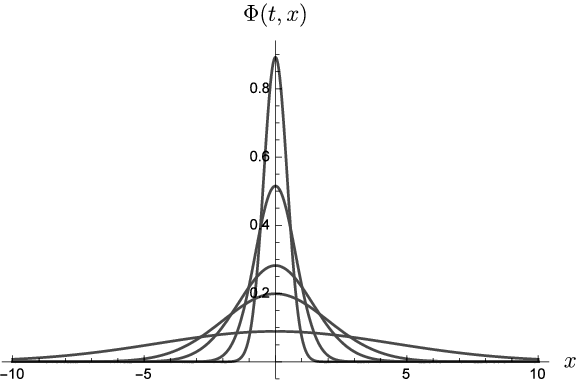
\includegraphics[width=8cm]{Fundamental-solution-to-the-heat-equation-at-different-time-moments-Note-that-if-t-0.png}
\label{Fundamental-solution-to-the-heat-equation-at-different-time-moments-Note-that-if-t-0}
\caption{भिन्न अवसरो पर ऊष्मा समीकरण का हल}
\end{figure}





\newpage
\section{सन्दर्भ ग्रन्थ}

Mathematical Physics, V. Balakrishnan, Ane Books Private Limited, 4281 Pranava Bhawan, 24 Ansari Road, Dariaganj, New Delhi - 110002



\end{document}
